\clearpage
\chapter{GPU Implementations}

In scientific computing, GPU programming can be hugely beneficial to large-scale problems. Due to the highly parallelisable architecture of GPUs, massive speed-ups can be seen. In this chapter, the heterogeneous, GPU programming model is discussed, as well as how this can be then implemented to apply the FEM. The design structure of the code written for this paper is detailed, as well as going through the theory of existing approaches.

\section{GPU Programming \& CUDA}

In GPU programming, there are multiple options currently available. Currently on Unix systems, the main two would be CUDA and openCL, others exist such as openGL and DirectX. They each have their own benefits, openCL is open source and can be used on any device with graphical processing abilities, from a phone to a cluster, while CUDA is only available solely for Nvidia devices. While all having their differences, they do all share the same general approach, this section details the model needed to program a GPGPU over a CPU.

\subsection{GPU Programming Model}\label{gpu_model}

\begin{figure}
	\centering
	\begin{subfigure}{0.35\linewidth}
		\centering
		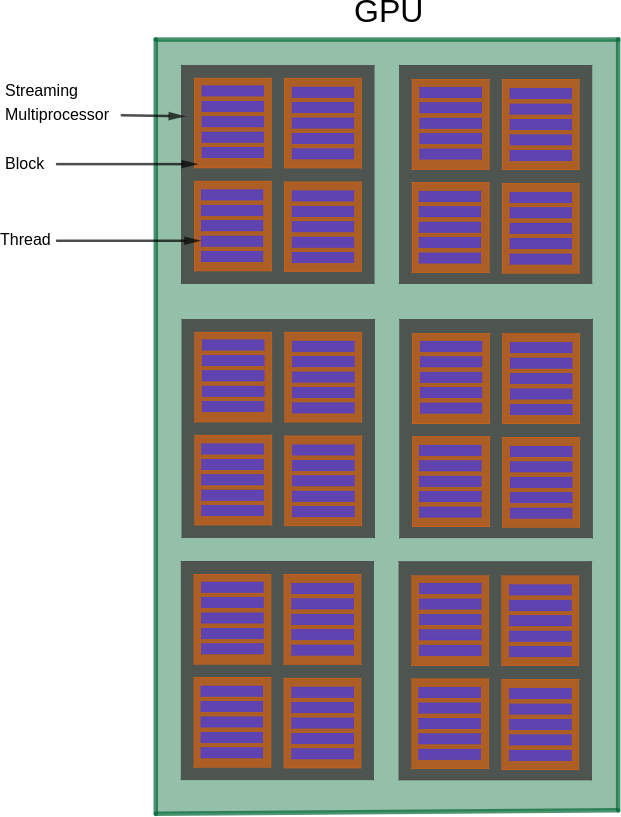
\includegraphics[width=\linewidth]{Figures/gpu_arch}
	\end{subfigure} \hfill
	\begin{subfigure}{0.55\linewidth}
		\centering
		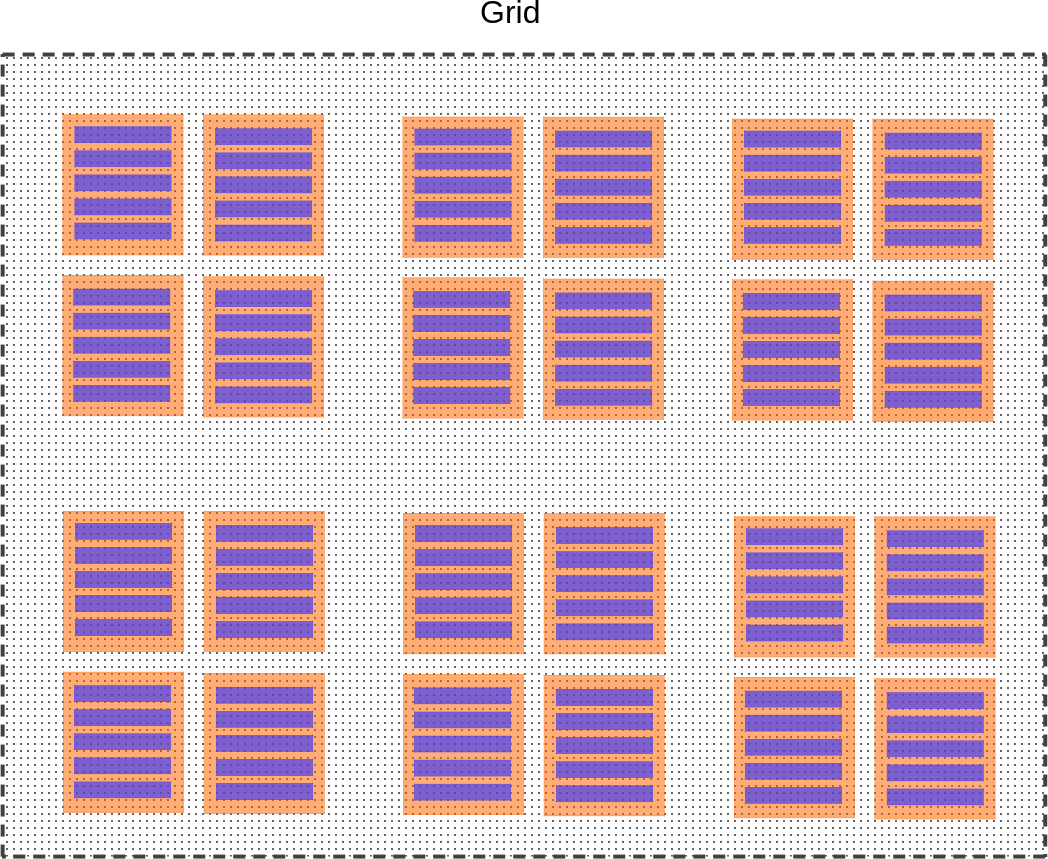
\includegraphics[width=0.9\linewidth]{Figures/gpu_grid}
	\end{subfigure}
	\caption{Illustration of a GPU's physical architecture and virtual 2D grid representation with dimensions $6\times4$ and block dimensions $5\times1$.}
	\label{fig:gpu_arch}
\end{figure}
While, as stated, GPUs have the potential to provide huge speed-ups, this is not necessarily a given. There is much to consider as a programmer when writing code which are not traditionally considered when writing code for CPUs - in serial, shared memory or even distributed architectures. CPUs traditionally consist of multiple cores, usually to the order of four to sixteen, sitting on a chip, with CISC architectures - meaning it is written to perform complicated instructions at high clock speeds. These chips often contain up to three levels of automated caches, with buffers, preventing thrashing by first-in-first-out or least-recently-used strategies. They regularly have extra chips called accelerators for performing specific calculations like cryptography or data compression and can have quite complex scheduling algorithms. In short, CPU chips are very clever, but fall down when it comes to high levels of parallelism.

GPUs, on the other hand, are made up of thousands of CUDA cores, sitting on what are known as Streaming Multiprocessors - often about eight or so per SM. Each of these SMs are arranged into blocks of threads, making up an overall grid. The threads inside each block are what allow these massive amounts of parallelisation. On the current Turing architectures, a block can have a max of up to 1024 threads per block, for example. Considering that there can be thousands of CUDA cores, it is now  how this can be hugely beneficial. Figure~\ref{fig:gpu_arch} shows this architectural design structure. So what is the downside? The first, and most evident thing to consider, is these cores are very basic. They have SIMD instruction sets, similar to RISC on CPUs, multiple less complex control units and have slower clock rates. GPUs do also have accelerators on them, such as the newer Tensor Cores and Ray Tracing cores, as seen in Figure~\ref{fig:turing} showing Nvidia's diagram of the Turing architecture, but these are relatively recent and not much used as of yet. Figure~\ref{fig:cpugpu} shows a relatively basic illustration of the difference in architectures, illustrating the larger, more complex control unit, shared cache as well as the much larger \textit{arithmetic logic units} - threads in a GPU's case.

\begin{figure}
	\centering
	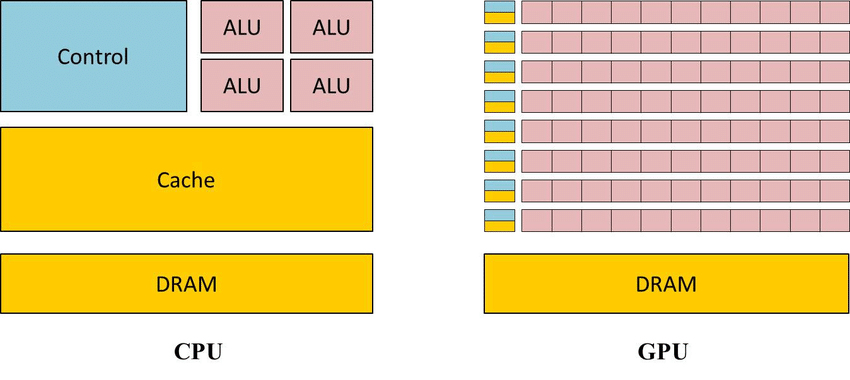
\includegraphics[width = 0.8\linewidth]{Figures/cpuvsgpu}
	\caption{Simplistic comparison of CPU versus GPU architectures.}
	\label{fig:cpugpu}
\end{figure}
\begin{figure}
	\centering
	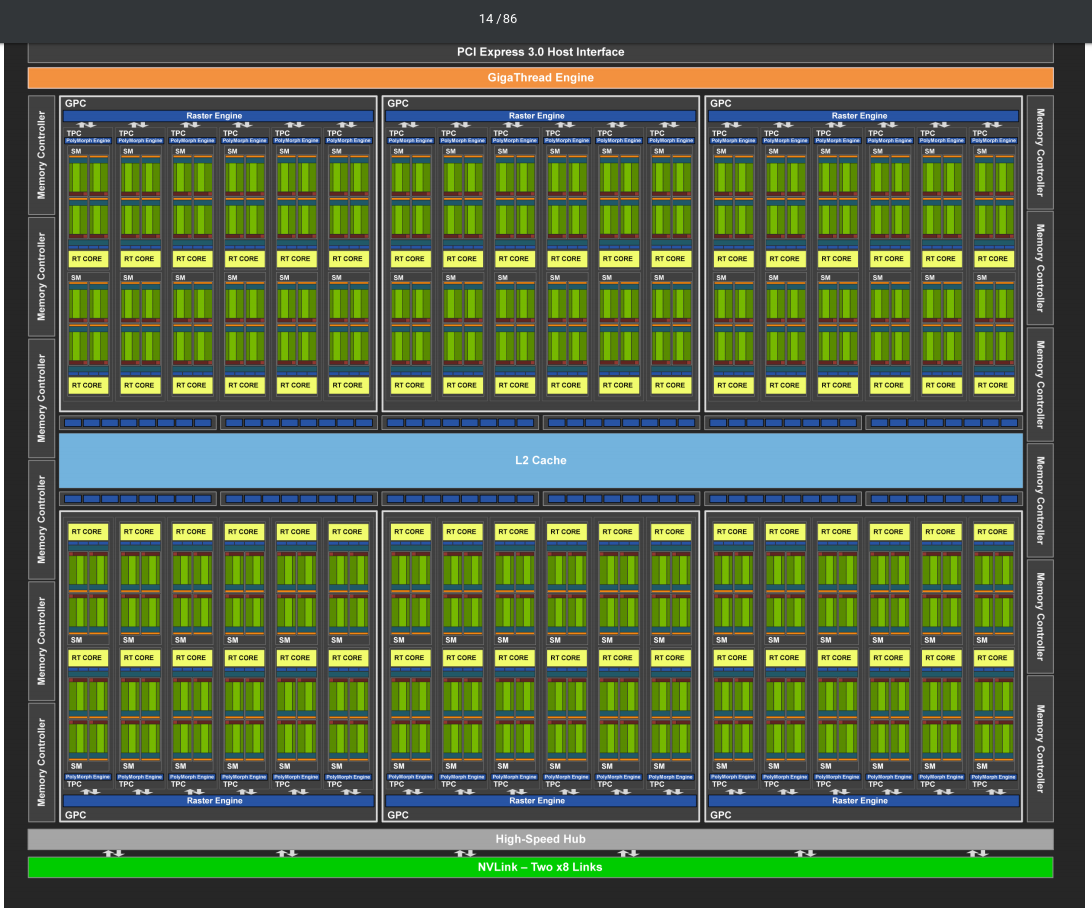
\includegraphics[width =0.65\linewidth]{Figures/turing}
	\caption{Illustration of Nvidia's current Turing architecture, showing its SMs and Ray Tracing cores.~\cite{turing}}
	\label{fig:turing}
\end{figure}

While slow clock-speed and simple instruction sets are the main drawbacks of using a GPU, there are other considerations to be made. The first, and almost certainly the most important when it comes to writing fast CUDA code is memory management. Unlike in Von Neumann, and other more modern CPU architectures, all of the memory management is left up to the programmer on a GPU and comes in various hierarchical levels. The largest bank of memory is \textit{global memory}, this is akin to the RAM of the GPU in terms of capacity order and is the slowest memory to access as it is physically furthest from the cores. The benefit of global memory is that it is both the largest and also accessible to all cores on the card. There are other faster memory banks such as constant, texture, and surface which have various advantages and disadvantages such as being closer to the chip but non-programmable once set et cetera. However, there are two main types of memory which are most advantageous to take advantage of, \textit{shared memory} and \textit{thread registers}. Register memory is stored per thread and sits physically on top of the core. It is as fast as one can possibly get, but is limited in size. Similarly, shared memory also sits on top of the core, the main difference is that shared memory is distributed across all threads in a given block and is usually around 48KB in modern architectures. Figure~\ref{fig:mem} illustrates the memory hierarchy on a GPU. Unlike in CPUs, the programmer must decide where the various data needed to run the program will be stored, so clearly managing this correctly will be hugely important.

\begin{figure}
	\centering
	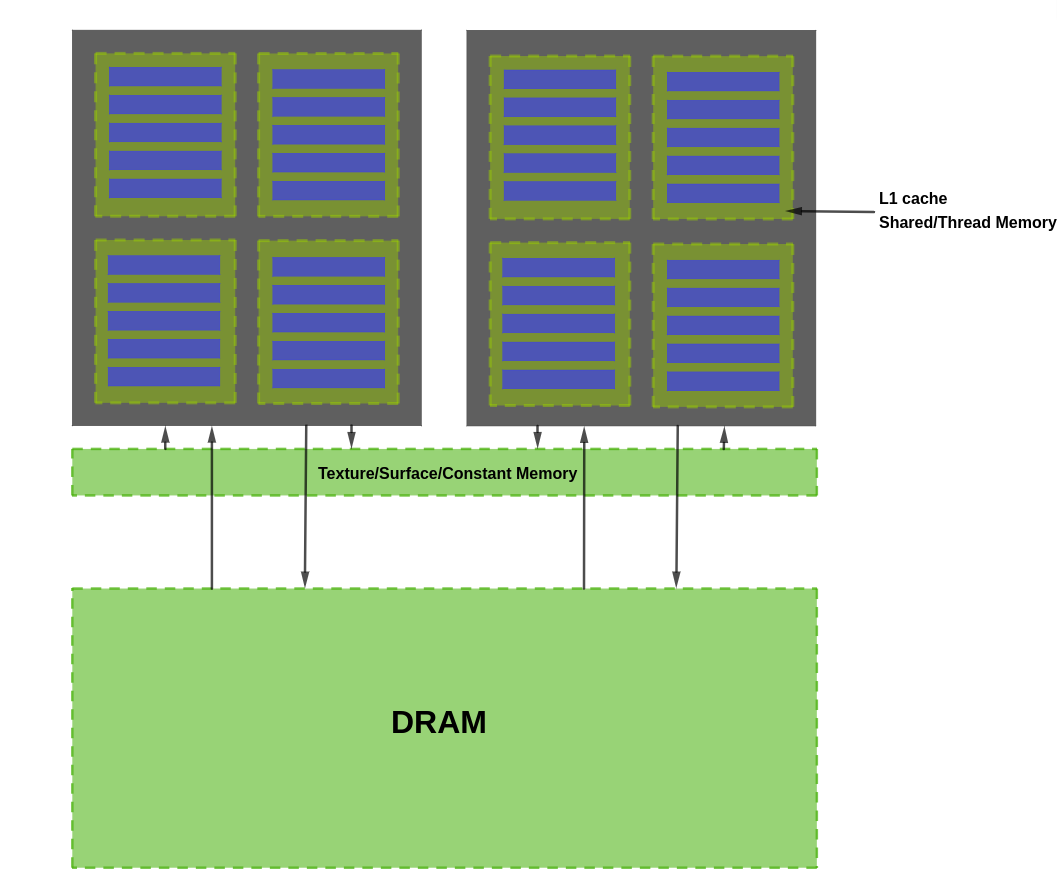
\includegraphics[width=0.8\linewidth]{Figures/mem_arch}
	\caption{Illustration of the memory structure on an Nvidia GPU.}
	\label{fig:mem}
\end{figure}

The final, main thing to consider, is what are known as warps. On the GPU, threads are organised into groups of 32. These groups of 32 threads all receive the same instructions at the same time. If some of the threads do not need to perform a given instruction, they will wait until the rest of the warp has completed the instruction until receiving another. Clearly, this can cause some bottlenecking. Figure~\ref{fig:warps} demonstrates how this can apply to a specific case. The best thing one can do when taking warps into consideration is to attempt to set block sizes as multiples of 32 - since usually blocks are all performing the same or similar instructions.

In terms of actually putting this all to use, in CUDA, the code is structured by splitting the functions up into three classifications:
\begin{enumerate}
	\item \texttt{\twound host\twound} functions, are functions executed on the CPU or host. These are usually left without being denoted.
	\item \texttt{\twound global\twound} functions, also known as kernels. These are invoked by the host, and are a way of initiating the CUDA code - these are executed on the GPU. Usual inputs into these include, block and grid dimensions, shared memory allocation and streams.
	\item \texttt{\twound device\twound} functions are GPU functions which are called on by the device - these cannot be called by the host.
\end{enumerate}
Clearly then, the main difference between programming on a CPU compared to on a GPU is the onus put on the programmer to manage scheduling and memory management amongst other things without the assistance of the device. Thus, CUDA code must inevitably be more basic and more-so a collection of simple executions - it lends itself best to large scale operations of basic calculations.
\begin{figure}
	\centering
	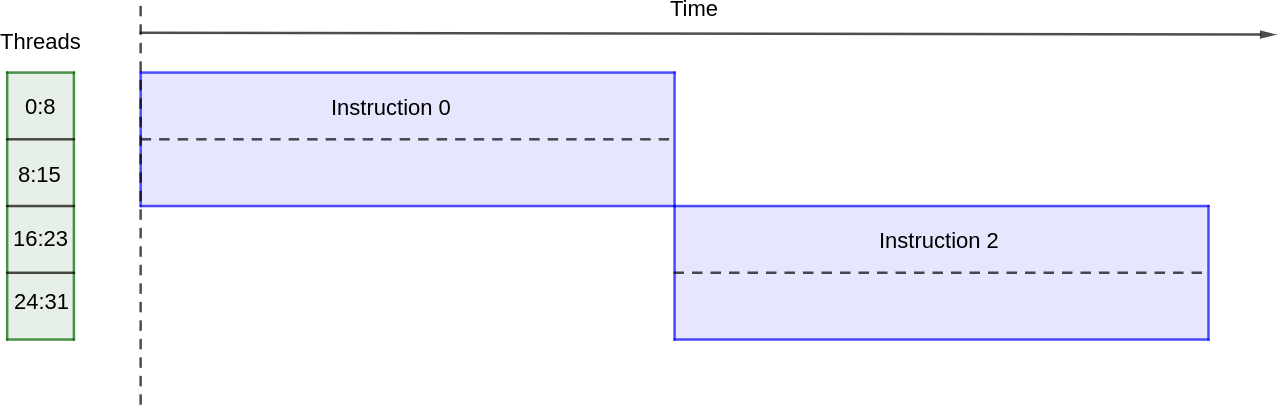
\includegraphics[width = 0.8\linewidth]{Figures/warps}
	\caption{Figure illustrating thread divergence for a single warp of size 32 when two instructions are issued for only certain threads in the warp.}
	\label{fig:warps}
\end{figure}

\subsection{CUDA Libraries}\label{culibs}

While many of the GPU programming variants like openCL and openGL have their pros and cons, the main reason for choosing CUDA for this paper is, for one, Nvidia cards were used for testing so the performance would be optimal, but more-so due to the extensive availability of libraries for CUDA - something which openCL does not have. Intel's MKL was discussed in Section~\ref{mkl}, and likewise, CUDA has its own collections libraries of mathematical functions. In Nvidia's case, these span from LAPACK, fast-Fourier transforms to image decomposition. In the case of this paper, cuBLAS, cuSOLVER and cuSPARSE were used. This is discussed in the breakdown of the GPU code's design structure in Section~\ref{culibs}. Similarly to the serial code, these were used for getting the Cholesky decomposition of a linear system and applying a direct solver. The cuBLAS package was used for finding the 2-norm of the error for each iteration seen in FEMSES.

\section{Current FEM Approaches}\label{approaches}

Currently, there are three existing methods of parallelising the finite element method and implementing it on a GPU:
\begin{itemize}
	\item Partitioning the linear system across the threads and solving.
	\item Applying a domain decomposition.~\cite{liu}
	\item Utilising multigrid techniques.~\cite{liu}
\end{itemize}
In this paper, the one implemented is the partitioning of the linear system across the processors and solving. This is, as it says on the tin; the element matrices and element vectors are assembled in parallel, the global stiffness matrix and stress vector are then also assembled across the threads in parallel, at which point this linear system is then solved using standard decomposition approaches. For this paper, the linear system decomposition was left to be handled by Nvidia's existing direct solver library cuSOLVER and the handling of the element matrices and assembly was implemented manually. These steps are no different really than discussed Section~\ref{approach}, barring needing to handle certain amounts of communication between threads handling nodes within the same cell, and also when mapping back to the global stiffness matrix/stress vector.

Domain decomposition is another technique applied to parallelising the FEM. The premise behind this approach is, if the mesh, or domain, $\Omega$, upon which the PDE is defined is decomposed into $n$ separate subdomains $\{\Omega_i\}_n$, these can each be solved iteratively using their own individual boundary conditions, as if they were independent PDEs. There are two main domain decomposition approaches, the Schwarz method for overlapping subdomains and the Schur method for disjoint domains. At each iteration there is corrections done on the locals boundary conditions via communication from neighbours and the iterations continue. This can often, be quite expensive in terms of computation costs, and depending on the architecture might not always be the optimal choice. For a GPU, due to the lack of being able to communicate between threads in separate blocks, this could cause some bottlenecks in the approach.

The final main approach to parallelising the FEM is by implementing a multigrid approach. The idea behind the multigrid approach is to coarsen the grid, and use interpolation to find estimates to this courser grid by iterating until convergence. This can then be refined using prolongation to make a finer mesh, of just the error from the previous prolonged mesh. This finer mesh can then have the same approach applied until convergence and the error prolonged again. This can oscillate up and down between fine and coarse grids until a converged solution is found. In the case of the FEM, this is a natural and efficient implementation as the entire domain can be divided into coarse and fine grids, each of which can be solved in parallel across the threads.
\section{FEMSES}

The finite element method single-element solutions (or FEMSES) approach is the key study in this paper.~\cite{femses} Developed with the aim of decoupling solutions to the element matrices, from assembling the global stiffness matrix, aiming to reduce a large computational cost from the existing methods seen in Section~\ref{approaches}.

Traditionally, the FEM has four main steps: create the mesh, generate the element matrices and element vectors, assemble the global stiffness matrix and stress vector and lastly, solve the linear system. Of course, the global stiffness matrix and stress vector can be quite a large linear system, the idea of FEMSES is to decouple this from the overall process by implementing a 2-step iterative relaxation scheme on the element matrices, applying a Jacobi iteration to get estimates of the local solutions, and then assembling these using a weighting to achieve an estimate of the global solution. This step is repeated until convergence, thereby relieving the need to assemble the global stiffness matrix. Once convergence is achieved, the global solution is passed back to the host in one single transfer. The approach is identical to ones seen previously up until the point of actually assembling the global stiffness matrix.

\subsection{Two-Step Iterative Relaxation}

The two-step iterative relaxation scheme is, naturally, going to be the most dominant kernel seen in the approach. However, the premise is that it should be more efficient than needing to apply the Cholesky decompositions and a direct solver on the entire system. Consider the Jacobi iterative scheme,
\begin{equation}
	x^{\text{(new)}} = M^{-1}(b - N x^{\text{(old)}}),
\end{equation}
for the linear system $Ax=b$, where $M = \text{diag}(A),~N=A-M$ is a matrix splitting. For our linear system for the FEM, $Lu = b$, now define local element solutions as $u_e$. If now, the Jacobi method is modified slightly, we can write it as,
\begin{equation}\label{jacobi}
	u^{\text{(new)}}_e = M^{-1}(b - N u^{\text{(old)}}).
\end{equation}
It may seem strange here, to have an estimate to the global solution on the RHS and a the local solutions' estimate on the left. However, failing this, what will result is  if one takes, for example, the Laplace equation where the RHS of the linear system $b$, is mostly sparse, barring cells which have boundary conditions, a collection of trivial matrices. The solution will be given for all internal cells as the initial and so in order to take account for the entire mesh, the global solution must be used for the RHS.

\begin{figure}
	\centering
	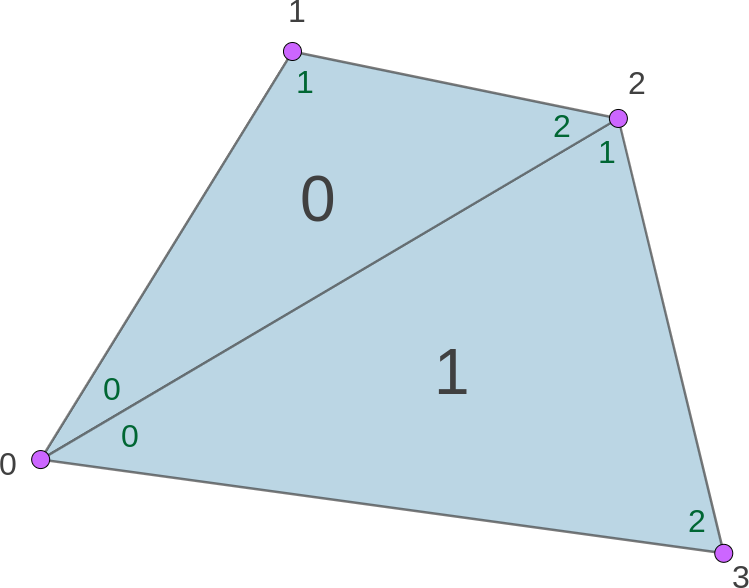
\includegraphics[width = 0.35\linewidth]{Figures/2cell2.png}
	\caption{Small two cell example of a mesh with global and local node numberings illustrated.}
	\label{fig:2cell2}
\end{figure}
The second step in the 2-step iterative relaxation is to take these local solutions, and assemble them into a global solution. This is done by creating a weighting array, summing up the contribution of each node on the denominator. Mathematically, the weighting and assembly is given by,
\begin{equation}\label{weight}
	u_i^{(new)} = \sum_e^{q(e,r) = i}\frac{A^{(e)}_{r,r}}{w_i} (u_r)_e^{(old)},
\end{equation}
where,
\begin{equation}
	w_i = \sum_e^{q(e,r) = i}A^{(e)}_{r,r}
\end{equation}
Figure~\ref{fig:2cell2} illustrates a small two-cell implementation. In this example, the Jacobi relaxation for cell 0 is given by,
\begin{equation}
	\left[\begin{matrix}
		(u_0)_e^{(new)} \\
		(u_1)_e^{(new)} \\
		(u_2)_e^{(new)}
	\end{matrix}\right] = 
	\left[\begin{matrix}
		\frac{1}{A^{(0)}_{0,0}} & 0 & 0 \\
		0 & \frac{1}{A^{(0)}_{1,1}} & 0 \\
		0 & 0 & \frac{1}{A^{(0)}_{2,2}}
	\end{matrix} \right]
	\times (-\mathbb{I}_3)
	\left[\begin{matrix}
		0 & A^{(0)}_{0,1} & A^{(0)}_{0,2} \\
		A^{(0)}_{1,0} & 0 & A^{(0)}_{1,2} \\
		A^{(0)}_{2,1} & A^{(0)}_{2,1} & 0 
	\end{matrix}\right]
	\left[\begin{matrix}
		u_0^{(old)} \\
		u_1^{(old)} \\
		u_3^{(old)}
	\end{matrix}\right]
\end{equation}
and the assembly using the weighting for global node 2,
\begin{equation}
	u_2 = \frac{A^{(0)}_{2,2}}{A^{(0)}_{2,2} + A^{(1)}_{1,1} } (u_2)_0 + \frac{A^{(1)}_{1,1}}{A^{(0)}_{2,2} + A^{(1)}_{1,1} } (u_1)_1.
\end{equation}

\subsection{Advantages \& Limitations}

The advantages of this approach is it improves on the parallelism seen in other methods. Of course, like the other approaches, the element matrices may be built in parallel and stored in global memory. However, after this, the assembly and solution of the linear system requires quite a substantial amount of communication between threads and synchronisation whereas the local solution estimates may be calculated entirely in parallel. The assembly of the global solution from the weightings can also be done substantially in parallel barring some scattered atomic functions when adding back to the global solution array. These atomic functions should not cause much overhead either as they are not in sequential order, they are ordered depending on the shape of the mesh. This is detailed in Section~\ref{femses}.

On the other hand, in terms of drawbacks, the Jacobi iteration isn't the most efficient iterative method. It bodes well here due to needing to use two different vectors on the LHS and RHS, which might cause some complications in something like the Gauss-Seidel, as you don't have the most recent update until the global solution is assembled. However, it is rather slow to converge. There is also somewhat of a communication hit in the process. After each iteration is completed, convergence must be checked, since kernels cannot call recursively, the convergence check must pass back the error term to the host, in order to test if the loop shall continue or not. It isn't hugely costly as it is only a single float, but it is still a consistent amount of device-host synchronisations.

\section{Implementations}\label{gpucode}

As mentioned, there is a lot of machinery and parts to move around in applying the FEM, especially when applying it on a GPU. Due to this, all of the code was written in CUDA~10.1, to avoid unnecessary complications with openCL and to take advantage of the Nvidia CUDA libraries. Unfortunately, CUDA cannot handle C++ code like the serial approach can, but rather only in C, thus the operations had to be made as simple as possible, no STL features were used in the CUDA code. 

\subsection{Design Structure}

Figure~\ref{fig:cuda} illustrates the overall design structure of the CUDA code. The code was largely divided up into three main files and headers:
\begin{enumerate}
	\item \texttt{gpu\_fem.cu} - Contains the \texttt{\twound host\twound} functions and all the \texttt{\twound global\twound} and \texttt{\twound device\twound} functions for the general, FEM GPU approach - applying a linear decomposition to the linear system.
	\item \texttt{gpu\_femses.cu} - Contains the \texttt{\twound host\twound} functions and all the \texttt{\twound global\twound} and \texttt{\twound device\twound} functions for the FEMSES GPU approach.
	\item \texttt{gpu\_utils.cu} - Contains general utility functions for use in the two main methods, such as LAPACK and BLAS operations.
\end{enumerate}
Both \texttt{\twound host\twound} functions are \texttt{extern} functions and so either can be invoked from the C++ code in \texttt{main.cc}. Note also that there is code reuse of \texttt{\twound device\twound} functions, so the flag \texttt{--relocatable-device-code=true} had to be set during compilation. Other flags for the CUDA libraries also had to be enabled, similar to the MKL library flags seen in the serial code.
\begin{figure}
	\centering
	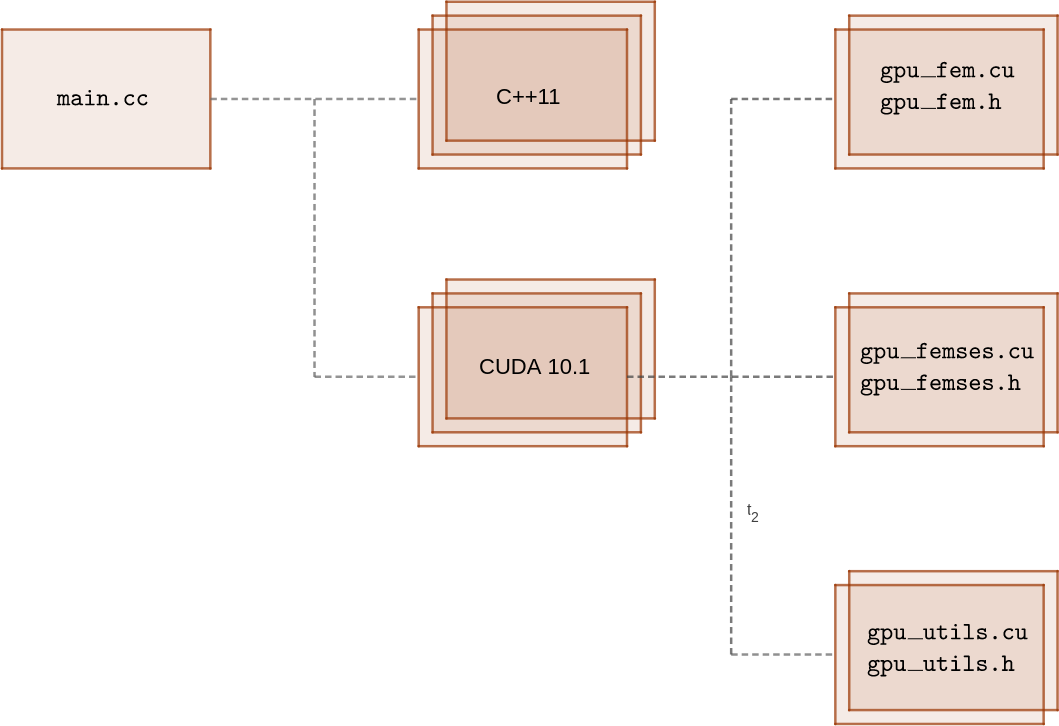
\includegraphics[width = 0.7\linewidth]{Figures/cuda_code}
	\caption{Structure of CUDA GPU code.}
	\label{fig:cuda}
\end{figure}

\subsection{Considerations}

There is a lot of data structures needed, so managing data reuse and reduction of transfers was a big consideration when designing the CUDA code. If something need not be transferred from host to device, it should be avoided. As well as this, the aim was to optimise shared memory use and minimise excessive synchronisation. For non-shared memory, attempting to keep the data coalesced is an important consideration as global memory access is quite slow. Fancy STL functionality couldn't be used so workarounds there had to be used - for example in the case of the sparsity pass function, this could not be performed on the GPU so it had to be done in serial and the resulting vectors transferred over. The last thing was to try minimise thread divergence from warps - reducing the amount of if statements is usually a good place to start along with making block sizes multiples of 32.

\subsection{Basic FEM}\label{basicfem}

\begin{figure}
	\centering
	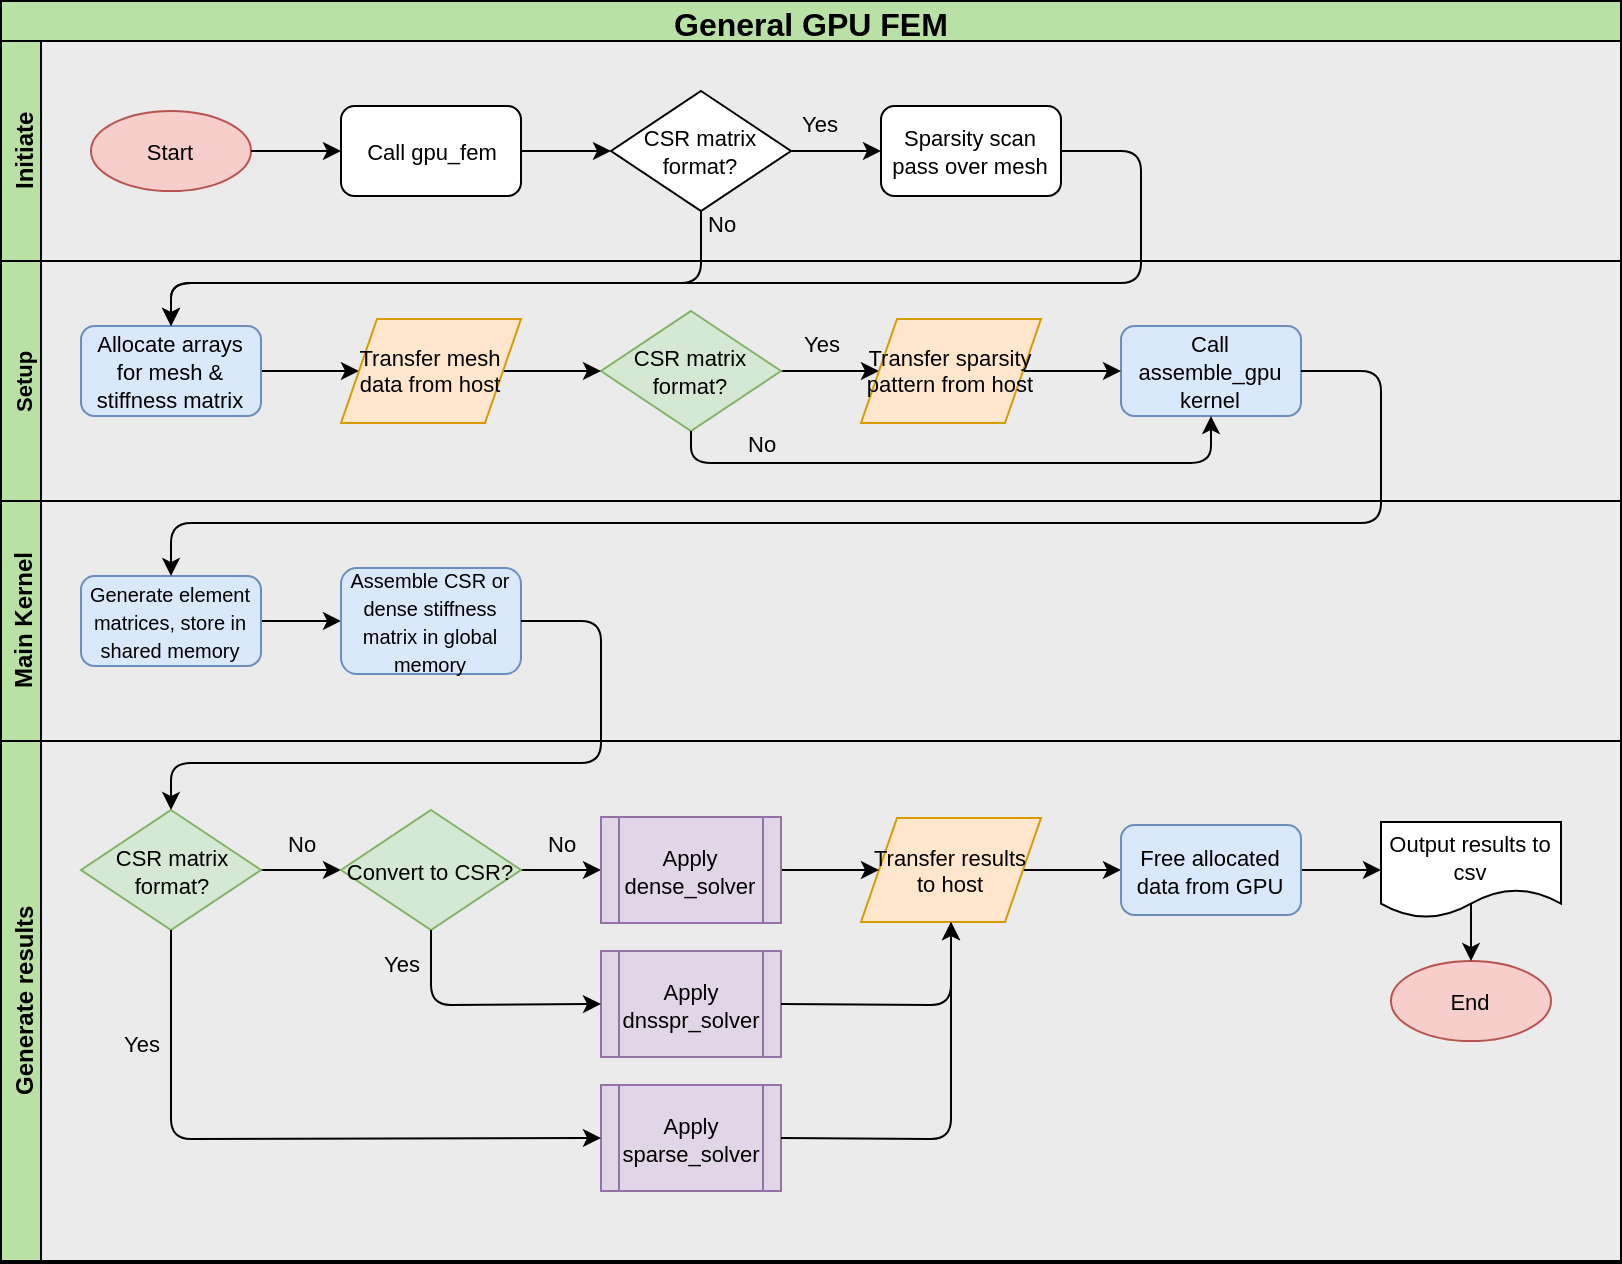
\includegraphics[width = 0.9\linewidth]{Figures/gpu_flowchart}
	\caption{Flowchart of general GPU FEM implementation.}
	\label{fig:gpu_flow}
\end{figure}
In Figure~\ref{fig:gpu_flow}, a flow chart of the approach taken to code a basic FEM implementation on a GPU is illustrated. The coloured steps are ones which are executed involving CUDA code, the white steps are ones which are executed entirely on the host. The generation of the mesh and all its pertaining information needed, is all completed in serial, which is then passed down to the device, and for the most part, barring a sparsity scan, the rest of the entire FEM process is completed on the device. The element matrices creation and stiffness matrix assembly is all completed in a single kernel. The linear system solution is then solved using cuSOLVER - and cuSPARSE depending on the matrix structure flagged at run-time. Once this is complete, the final solution is passed back to the host and the CUDA code is complete.

\subsubsection{Storage \& Memory Management - Mention solver taking up space}

\begin{figure}
	\centering
	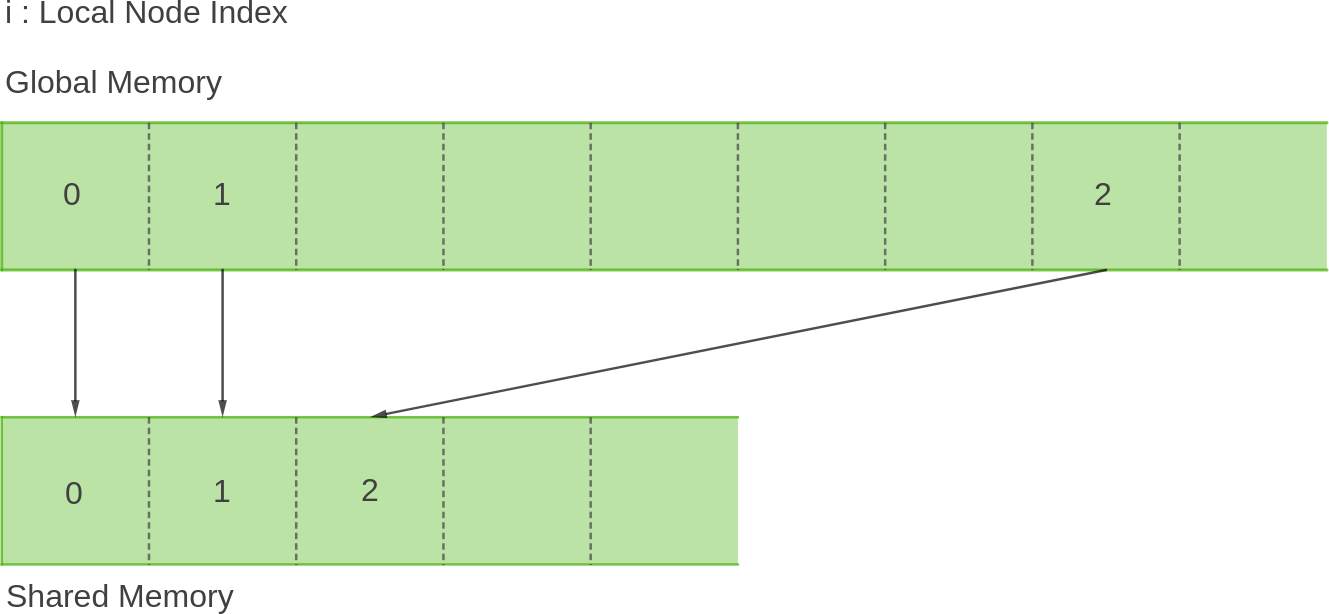
\includegraphics[width = 0.8\linewidth]{Figures/non_coalesced}
	\caption{Illustration of global memory random access pattern being transferred to shared memory to ensure coalescence.}
	\label{fig:coalesc}
\end{figure}
In terms of storage, for a problem which scales like FEM does, managing one's resources correctly and not doing excessive memory allocations is important - along with, of course, freeing any allocations which are completed. The first thing needed to be allocated on the GPU is the five arrays to store the mesh. Exactly like was mentioned in Section~\ref{mesh}, memory needs to be allocated to store \texttt{vetices\_gpu}, \texttt{cells\_gpu}, \texttt{dof\_gpu}, \texttt{is\_bound\_gpu} and \texttt{bdry\_vals\_gpu}. In terms of memory being coalesced, all five arrays are indeed contiguous, and in both \texttt{cells\_gpu} and \texttt{dof\_gpu}, the memory access pattern is sequential so this won't pose any coalescence problems. However, the other three arrays, the memory access pattern jumps up and down the array, completely dependent on the shape of the mesh, and the connectivity of the nodes. Thus to handle this, as detailed in the device functions, the necessary values are read into shared memory in single writes to hedge this bottleneck. Figure~\ref{fig:coalesc} illustrates this, showing the lack of coalescence and the solution by writing to shared memory once.

Naturally, the next thing which needs to be allocated is the actual stiffness matrix itself. For this, unlike in serial, only the global stiffness matrix and stress vector need be allocated on global memory, since the local element matrices will be stored on shared memory. Depending on the choice to assemble a sparse or dense matrix will decide what must be allocated. For a dense case, a single dimensional array \texttt{L}, will be allocated, for the sparse case, three arrays must be allocated, \texttt{valsL}, \texttt{colIndL} and \texttt{rowPtrL}, as seen in Section~\ref{sparse}. The CSR matrix, unfortunately does not have coalesced memory access, but it makes up for this by the huge reduction in the actual size of the matrix, and so, the timing should scale far better than dense. Both dense and sparse allocated the same space for the stress vector, as it is stored in dense format. This will be overwritten with the resulting solution, saving the space for needing an extra array.

There is quite a large amount of data needed to be transferred from the offset in the FEM from device. All five of the mesh's arrays must be transferred from host to device (\texttt{dof\_gpu} technically does not when using P1 cases, but as stated this is to leave scope for further expansion). On top of this, as mentioned, the GPU cannot perform the sparsity scan algorithm, thus this must be done on the host. This algorithm populates both the column-index array and row-pointer array in the CSR structure, both of these must be transferred at the beginning when a sparse solution is chosen.

In terms of transfers, in both sparse and dense cases, the five arrays for the mesh need to be transferred. If \texttt{order} and \texttt{num\_cells} represent the number of unknowns/nodes and the number of cells respectively, then these five arrays take up,
\begin{flalign}\label{mem}
	\texttt{mem} &= \texttt{(3}\times\texttt{order}\times\texttt{sizeof(float))+(((6}\times\texttt{num\_cells)+order)}\times\texttt{sizeof(int))},&&\\
	\texttt{mem} &= \texttt{(14}\times\texttt{order) + (12}\times\texttt{num\_cells)},&&
\end{flalign}
where \texttt{mem} is measured in bytes. The two approaches  will then differ when it comes to storing the stiffness matrix and transfers. For both cases, the global solution array will need to be stored and also transferred back to the host, which will take up $\texttt{order}\times\texttt{sizeof(float)}$, or $\texttt{4}\times\texttt{order}$, bytes. This is the same array used to store the stress vector - it will simply be overwritten by the solution. For transfers, the sparse matrix must receive two arrays from the host after the sparsity pattern has been completed, the column-index array and row-pointer array, these are sized $\texttt{nnz}\times\texttt{sizeof(int)}$ and $\texttt{(order+1)}\times\texttt{sizeof(int)}$ respectively, where \texttt{nnz} is the number of non-zero entries achieved from the sparsity scan. The sparse approach also must store the values in \texttt{valsL}, taking up $\texttt{nnz}\times\texttt{sizeof(float)}$ too. There are no extra transfers needed for the dense approach but the memory needed to store the stiffness matrix is far larger, coming in at $\texttt{order}\times\texttt{order}\times\texttt{sizeof(float)}$. Therefore it can be said that the total amount of data needed to be transferred,
\begin{flalign}
	&\texttt{mem\_transf\_sparse} = \texttt{(20}\times\texttt{order) + (12}\times\texttt{num\_cells) + (2}\times\texttt{nnz) + 2},&& \\
	&\texttt{mem\_transf\_dense} = \texttt{(18}\times\texttt{order) + (12}\times\texttt{num\_cells)}, &&
\end{flalign}
and the total amount of memory allocated on global memory,
\begin{flalign}
	&\texttt{mem\_alloc\_sparse} = \texttt{(20}\times\texttt{order) + (12}\times\texttt{num\_cells) + (2}\times\texttt{nnz) + 2},&&\\
	&\texttt{mem\_alloc\_dense} = \texttt{(18}\times\texttt{order) + (12}\times\texttt{num\_cells) + (4}\times\texttt{order}\times\texttt{order)}.&&
\end{flalign}
This is an important factor to take into account when deciding what problem size to calculate as memory on the GPU is limited. In the case of the two GPUs tested in this report, the Tesla K40 has 12GB of global memory, while the GeForce RTX2080 Super has 8GB.

\subsubsection{Kernels}

There are two main kernels for this approach: the first kernel, \texttt{assemble\_gpu} or in its sparse form, \texttt{assemble\_gpu\_csr}, will take the input mesh as transferred prior, create the element matrices and assemble the global linear system, storing it back into global memory, this is demonstrated in Listing~\ref{lst:fem_main}; the second kernel, utilises CUDA libraries to solve the linear system. The assembly kernel was written specifically for this implementation, thus the setup of the grid and block dimensions must be set by the user. In order to take as much advantage of shared memory as possible, it was noted that the only real communication at this stage in the FEM process, is between nodes in the same cell. The setup of the kernel is then set that there are \texttt{block\_size\_X}, cells per block, in the $x$ direction, and 3 nodes per cell, in the $y$ direction. This gave the convenient benefit of \texttt{idx} being equal to the cell number, and \texttt{idy} being the local node numbering. The kernel itself, runs two primary device functions, the first one generates the element matrices on shared memory, and the second then assembles these from shared memory into the global stiffness matrix, writing back to global memory. For two reasons, this is where the kernel had to terminate: you cannot globally synchronise the entire CUDA device within a kernel, only individual blocks, moving on to solve the linear system from here would almost certainly cause race conditions. The second reason is simply to avoid having to rewrite linear solver libraries that have already been optimised.

The linear solver kernel, comes in three different variations: one for CSR, one for dense matrices, and one which converts a dense matrix into CSR and solves. Unlike the assembly kernel, however, there is no need to decide how to organise the blocks and threads as this is taken care of by the library itself inside a variable called the handle, which is invoked at the beginning and passed into all library functions. In terms of what actual library functions are used, for the sparse solver, cuSPARSE is used to define the matrix structure, such as number of non-zeros, zero-based indexing, symmetric positive definite et cetera. This is used in tandem with cuSOLVER's single-precision, sparse SPD, Cholesky decomposition direct solver, \texttt{cusolverSpScsrlsvchol}. Unlike in the serial version, and Intel's DSS, the cuSOLVER kernel needs to store the entire matrix, as opposed to only the upper or lower half. This is an unnecessary bottleneck but one which cannot be avoided. The dense-CSR solver kernel, applies the same functionality as the sparse kernel, except for executing two other library kernels prior to the solver, \texttt{cusparseSnnz}, to deduce the sparsity pattern of the matrix, and \texttt{cusparseSdense2csr}, to convert from dense to CSR. The dense solver on the other hand, naturally does not use cuSPARSE. It does, however, split its solver kernel into two separate operations, the first being the actual Cholesky factorisation using \texttt{cusolverDnSpotrf} and the second applies the solver, \texttt{cusolverDnpotrs}. Figure~\ref{fig:cusolvers} shows flowcharts of the necessary steps required in order to execute the three solver variants.

\begin{lstlisting}[style=cppStyle,caption={Main kernel in general FEM approach to generate element matrices and assemble global linear system.},label={lst:fem_main}]
__global__ void assemble_gpu(
                float *L, 
                float *b, 
                float *vertices, 
                int *cells, 
                int *is_bound, 
                float *bdry_vals, 
                int order,
                int num_cells)
{
	   // idx = cell number
    int idx = blockIdx.x * blockDim.x + threadIdx.x ;
    // idy = local node number
    int idy = blockIdx.y * blockDim.y + threadIdx.y ;
    // shared mem to store elem mats & constants
    extern __shared__ float temp1[];

    if(idx < num_cells && idy < blockDim.y ){

       assemble_elem(vertices, cells, is_bound, bdry_vals, temp1, idx, idy);
       __syncthreads();
       assemble_mat(L, b, vertices, cells, temp1, idx, idy, order);
    }
}
\end{lstlisting}
\begin{figure}
	\centering
	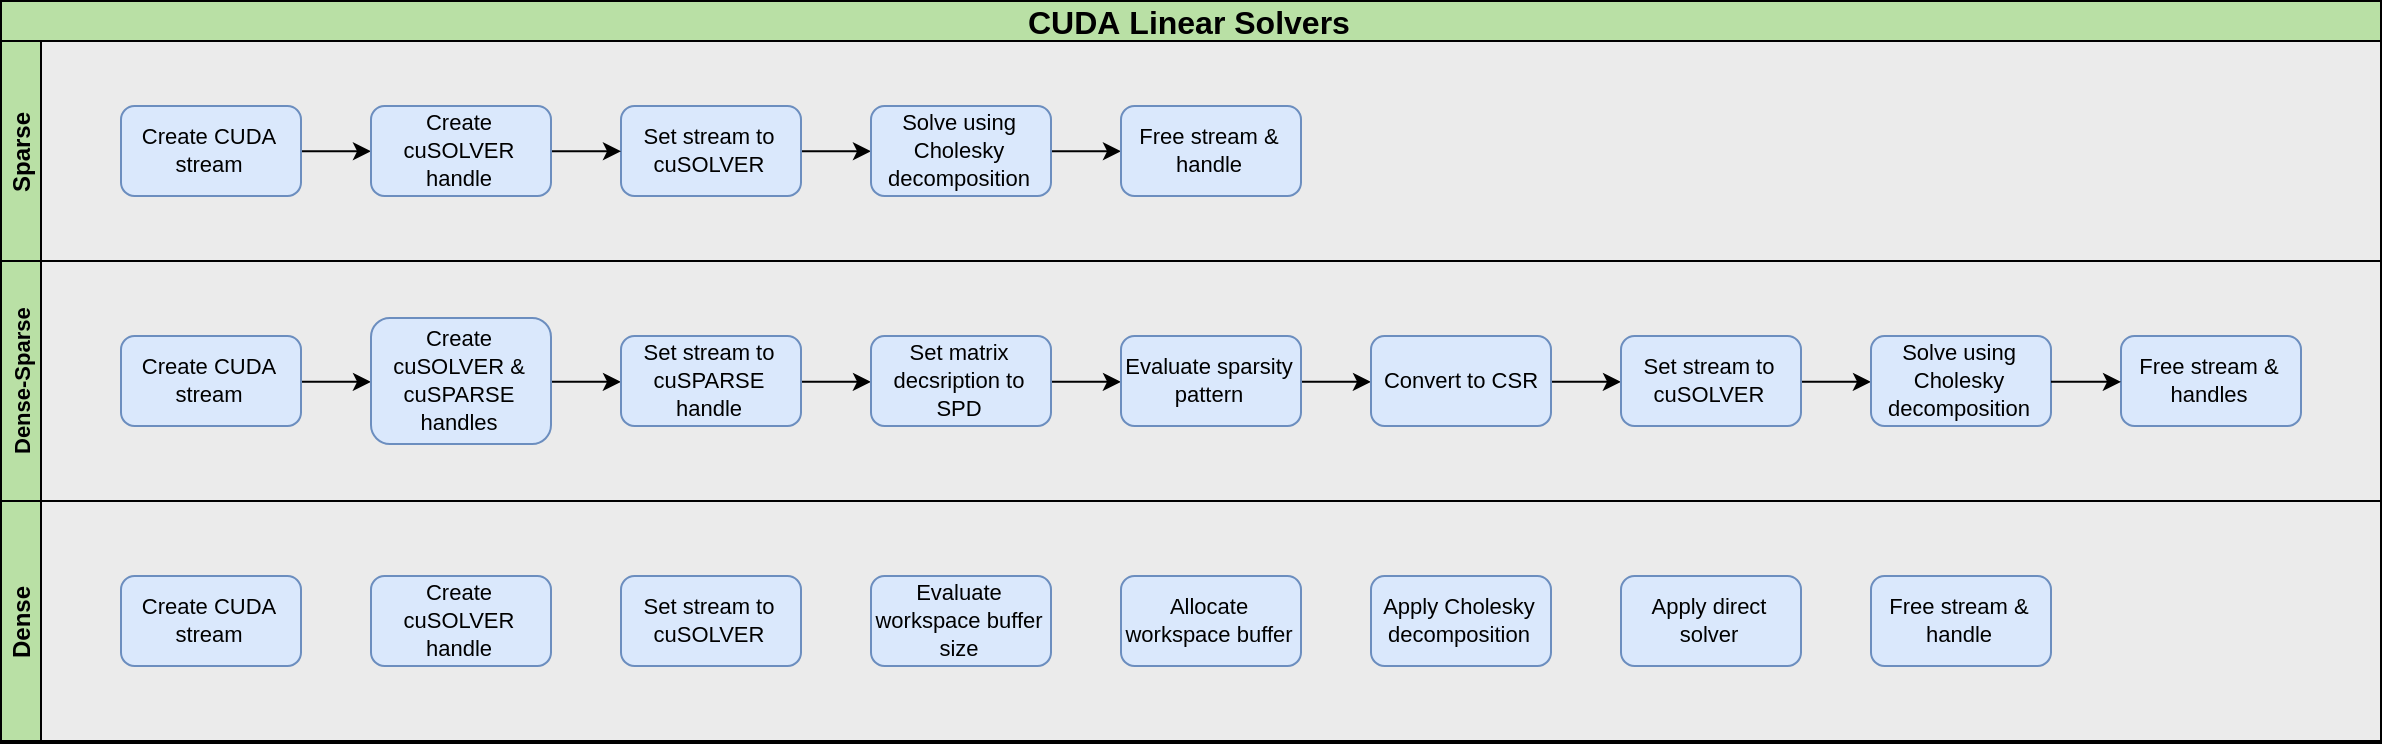
\includegraphics[width=0.9\linewidth]{Figures/cuda_solvers}
	\caption{Flowchart illustrating the steps needed to implement solvers from CUDA's linear algebra libraries.}
	\label{fig:cusolvers}
\end{figure}

\subsubsection{Device Functions}

There are two main device functions written for the assembly kernel. Prior to running these, when invoking the kernel the required amount of shared memory must be allocated. The grid structure is defined as \texttt{block\_size\_X} FEM cells per block, within each block there is one FEM cell designated per row of threads in the $x$-axis, and 3 nodes per row i.e. one node per thread in the $y$-axis. The shared memory needs to be large enough to store the element matrix \texttt{Le}, the element vector \texttt{be} as well as some other constants which need reuse such as the coordinates of each node in the cell \texttt{xi}, the global node numberings \texttt{dof\_r} and the constants seen in Equation~\eqref{conv}, for each cell in the block. Thus the amount of shared memory required is $\texttt{28}\times\texttt{block\_size\_X}$. This memory structure is displayed in Figure~\ref{fig:shared_mem} for an example block size of 4 in the $x$-axis. This would need to be larger of course, for non-P1 type problems but for this implementation it is sufficient.

\begin{figure}
	\centering
	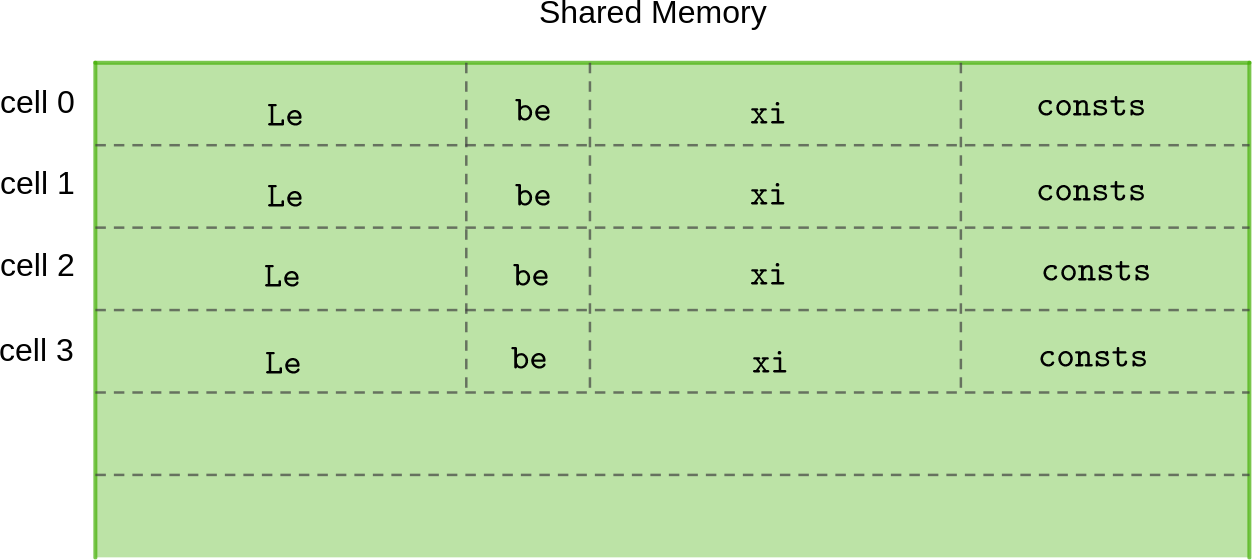
\includegraphics[width = 0.75\linewidth]{Figures/shared_pos}
	\caption{Illustration of shared memory structure for assembly kernel for a block containing four cells of the mesh.}
	\label{fig:shared_mem}
\end{figure}

The first device function, \texttt{assemble\_elem}, starts off by setting pointer values for the element matrices, element vectors and constants in shared memory. It reads in the global node numbering associated with the node for that particular thread into the thread register. It then reads in the coordinates of the three nodes in that cell into shared memory so that data is now coalesced and then synchronises the threads in the block. The area of the cell is calculated by the thread associated with local node 0, and then the $\beta$ and $\gamma$ values are calculated in parallel. After this point, the device function runs Algorithm~\ref{algo:elems}, where each thread calculates a single row in the element matrix and writes them to the shared memory array. Notice that there is need for atomic functions when enforcing the boundary conditions, this is to prevent race conditions as the threads need to write to the same memory addresses. 

A large speed-up point here is that the element matrices never need to be written to global memory, but rather the second kernel which assembles the global stiffness matrix simply assigns the pointers to the same location as the previous device function. For the assembly function, the global node numbers for the node associated with each thread are read in from global memory once and written over the constants in the previous function. Algorithm~\ref{algo:assemble} or Algorithm~\ref{algo:assemble_csr}, is then applied in parallel, depending on whether the matrix is dense or CSR, and written back to global memory. Again, unlike in the serial case, for the CSR matrix the entire matrix must be assembled and not simply its upper or lower-echelon form due to limitations of cuSOLVER.

\subsection{FEMSES}\label{femses}

\begin{figure}
	\centering
	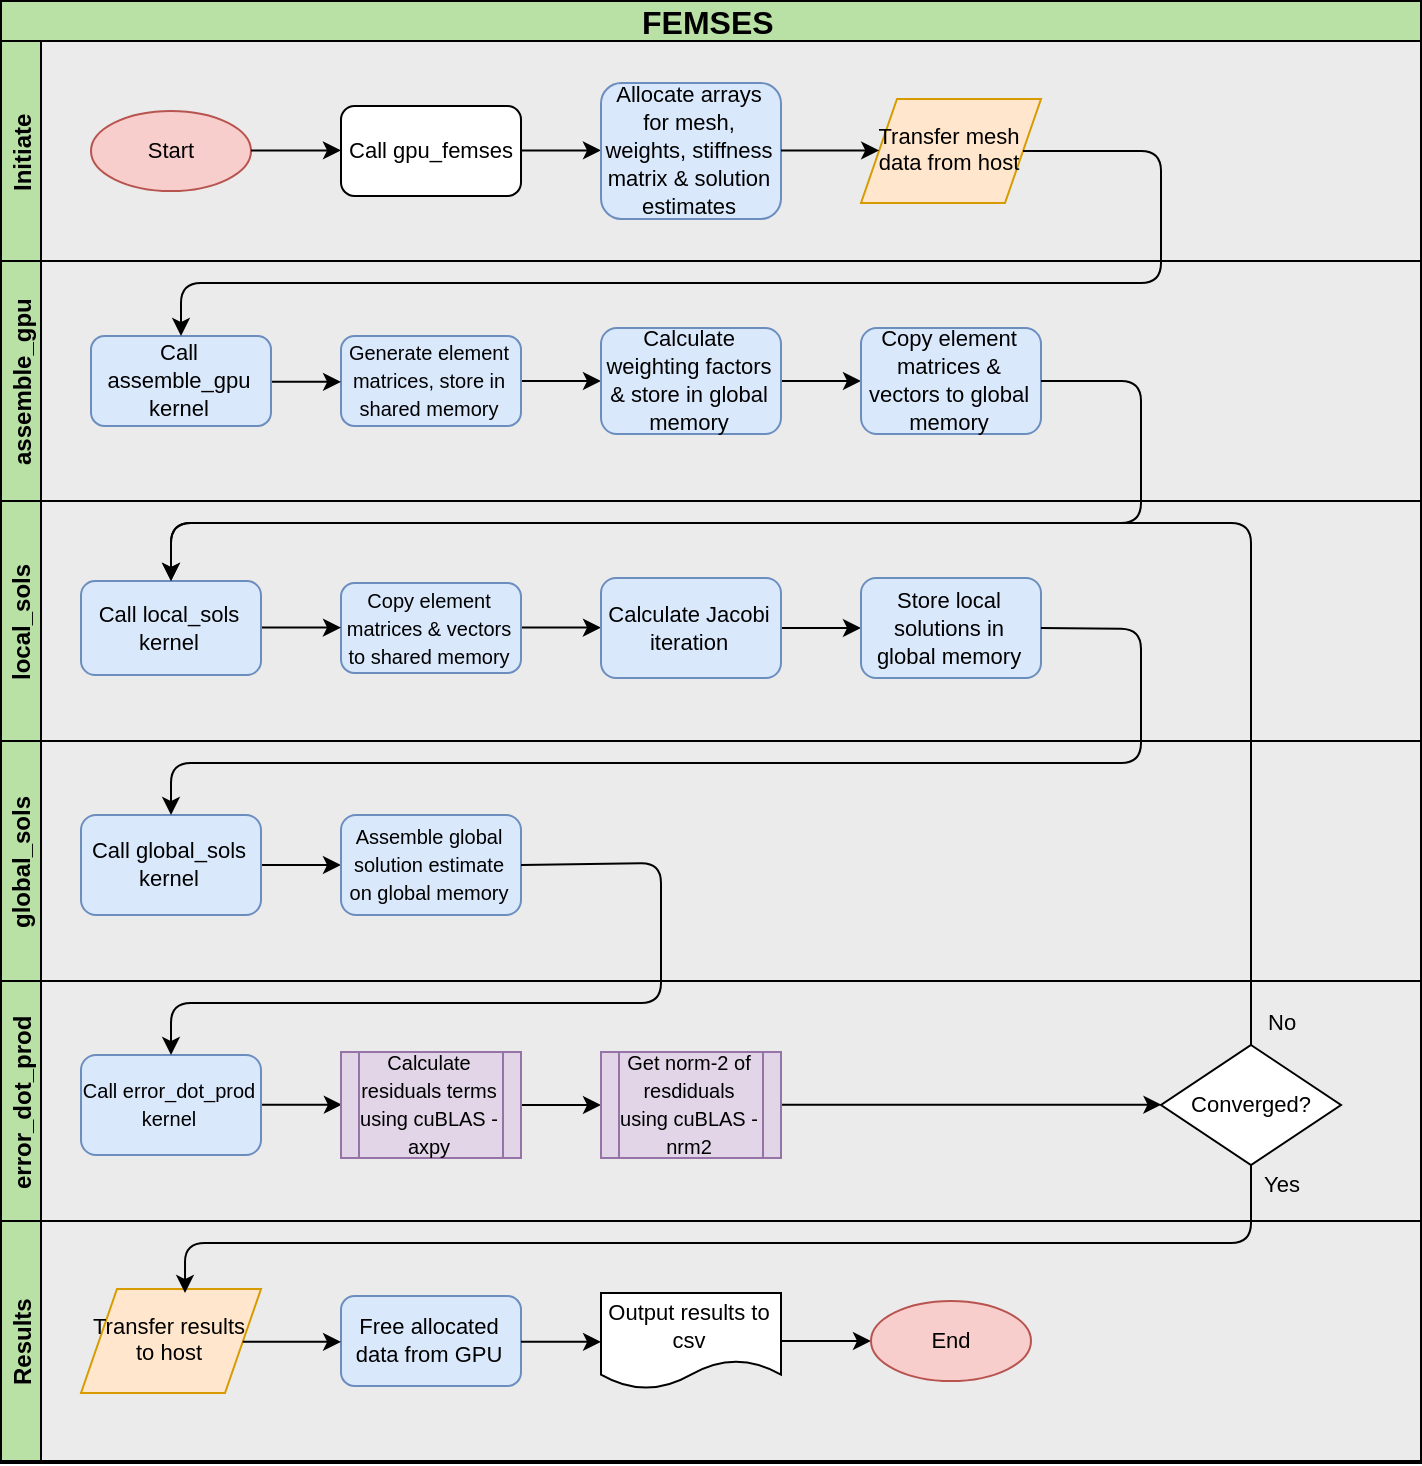
\includegraphics[width=0.9\linewidth]{Figures/femses_flow}
	\caption{Flowchart of FEMSES approach.}
	\label{fig:femsesflow}
\end{figure}

Figure~\ref{fig:femsesflow} shows a float chart of the FEMSES process when applied with CUDA code. Like before, the coloured steps are carried out by/on the GPU, the white are the host C++ functions. Unlike in Fernandez~\cite{femses}, the assembly of the element matrices is carried out on the GPU, and stored into global memory instead of being transferred by the host to device - this should show some speed-ups over the results seen. Just like in the standard FEM implementation, all the mesh creation operations are carried out on the host and transferred down, in this case excluding the sparsity scan as there is no global matrix ever assembled in this method. The kernels are divided up in quite a logical manner, but this is simply due to synchronisation limitations on the CUDA cores. Everything that can be completed in a single kernel without needing a global synchronisation, is completed as such. Unfortunately, any point that needs global memory synchronisation, will require a kernel to terminate. This can be seen in the flow chart, where the element matrices are assembled and stored into global memory, and using these, local solutions are calculated using the Jacobi relaxation and stored into global memory. Following that, another kernel assembles the global solution, again writing back to global memory. Lastly, cuBLAS is called in order to calculate the 2-norm of the error and check for convergence. Clearly at each of these steps, global memory must synchronise and so there was no option but to write these all in separate kernels.

\subsubsection{Storage \& Memory Management}

The FEMSES approaches shares the exact same memory allocations as the standard GPU FEM approach does, when it comes to allocating for the mesh. The same five arrays must be allocated and transferred taking up an identical amount of bytes as Equation~\eqref{mem}. After this point though, the two differ. Clearly, since the aim of the FEMSES approach is to avoid generating a global stiffness matrix and stress vector, then there will be no need to allocate space for them. Instead rather, two arrays must be allocated, both containing all of the element matrices and element vectors, \texttt{Le},\texttt{be} - these will be of size $\texttt{num\_cells}\times\texttt{9}\times\texttt{sizeof(float)}$ and $\texttt{num\_cells}\times\texttt{3}\times\texttt{sizeof(float)}$. There must also be space allocated to store an array of all the local element solutions \texttt{ue}, for when they are written back from shared memory, which is the same size as \texttt{be}. Finally there must be memory allocated to store both previous and new global solution estimates in the iteration, \texttt{up\_gpu}, \texttt{un\_gpu}, and an array containing the denominator of all the weightings, \texttt{w}  as seen in Equation~\eqref{weight} - all three of these are size $\texttt{order}\times\texttt{sizeof(float)}$ each. In total then, the global memory needed to perform FEMSES is,
\begin{flalign}
	\texttt{mem\_alloc\_femses} = \texttt({26}\times\texttt{order) + (72}\times\texttt{num\_cells)}. &&
\end{flalign}

For transfers, all of the data that is allocated besides the mesh is calculated on the GPU, and only the resulting global solution needs to be transferred. Besides this, there is also one single float transferred at every iteration to check for convergence, of course this is not known a priori so for arguments sake, if there is \texttt{iter} iterations before convergence then the total data transferred is,
\begin{flalign}
	&\texttt{mem\_transf\_femses} = \texttt{(18}\times\texttt{order) + (12}\times\texttt{num\_cells) + (4}\times\texttt{iter)}. &&
\end{flalign}

\subsubsection{Kernels}

The FEMSES approach is divided up into four component kernels as seen in Figure~\ref{fig:femsesflow}:
\begin{enumerate}
	\item generate element matrices.
	\item calculate local element solutions.
	\item assemble global solution estimate.
	\item calculate 2-norm of error.
\end{enumerate}
In the cases of the first three kernels, the grid structure is identical to what was seen in the general FEM approach, allowing maximum use of shared memory and attempts to prevent thread divergence.

The first kernel, listed in Listing~\ref{lst:femses_main}, is called on to generate the element matrices. It uses the same device function as the main kernel in the alternate approach to generate the element matrices on shared memory. After this, it calls on a device function to calculate the weightings and save them onto global memory. Lastly it writes the element matrices and element vectors to the array in global memory and terminates the kernel.
\begin{lstlisting}[style=cppStyle,caption={Initial kernel in FEMSES to generate element matrices and store in global memory.},label={lst:femses_main}]
__global__ void assemble_elems_gpu(
                float *Le, 
                float *be, 
                float *w,
                float *u_glob,
                float *vertices, 
                int *cells, 
                int *is_bound, 
                float *bdry_vals,
                int order,
                int num_cells)
{
	   // idx = cell number
    int idx = blockIdx.x*blockDim.x + threadIdx.x;
    // idy = local node number
    int idy = blockIdx.y*blockDim.y + threadIdx.y;
    extern __shared__ float temp1[];

    if(idx < num_cells && idy < blockDim.y){
        // __device__ fn taken from other header to avoid code-reuse //
        assemble_elem(vertices, cells, is_bound, bdry_vals, temp1, idx, idy);
        __syncthreads();
        calc_weights(w, cells, temp1, idx, idy);
        elems_glob_cpy(Le, be, temp1, idx, idy);
    }
    // assigning initial guess for Jacobi to 0.0 
    if( (idx*3) + idy < order){
        u_glob[(idx*3) + idy] = 1.0;
    }
}
\end{lstlisting}

The second kernel, evaluates the local solution estimates. Illustrated in Listing~\ref{lst:local}, this has two main device functions: the first reads in the element matrices and element vectors from global to shared memory. The second device function is the key computational step of this approach, calculating the Jacobi iteration estimate, as seen in Equation~\eqref{jacobi}, to generate local solutions and writes these back to global memory.
\begin{lstlisting}[style=cppStyle, caption = {Kernel to evaluate local solutions in FEMSES using Jacobi iteration.}, label={lst:local}]
__global__ void local_sols(
                float *Le,
                float *be,
                float *ue,
                float *up_glob,
                int *cells,
                int num_cells)
{
    int idx = blockIdx.x*blockDim.x + threadIdx.x;
    int idy = blockIdx.y*blockDim.y + threadIdx.y;
    extern __shared__ float temp1[]; 

    if(idx < num_cells && idy < blockDim.y){
        elems_shared_cpy(Le, be, temp1, idx, idy);
        __syncthreads();
        jacobi_iter(ue, up_glob, cells, temp1, idx, idy);
    }
}
\end{lstlisting}

The final purpose-written kernel in this method assembles the global solution array using the weightings. Seen in Listing~\ref{lst:global}, there was in fact no need for extra device functions here simply due to the fact that it was a read/write operation and one line of calculation - an atomic addition did sufficiently here. Thankfully, due to the irregular memory access pattern the atomic add should not actually pose much bottleneck. In Fernandez~\cite{femses}, the residuals were also calculated in this kernel, which is believed to be an oversight or error since this will potentially cause a race  condition as there is no guarantee the entire global solution has been assembled until the kernel terminates.

The final calculation kernel here is utilising cuBLAS. The kernel uses two BLAS Level-1 operations, the first being the vector product, $y \leftarrow \alpha x + y$, or \texttt{cublasSaxpy}, to evaluate the residual vector and write it over $y$. The second operation evaluates the 2-norm of the residual, $e \leftarrow \sqrt{\langle r, r\rangle}$, or \texttt{cublasSnrm2}. The resulting error term is passed back to the device.

\begin{lstlisting}[style=cppStyle, caption={Kernel to assemble global solution vector in FEMSES from local solution estimates using weighting.}, label={lst:global}]
__global__ void glob_sols(
                float *Le, 
                float *w, 
                float *u_glob, 
                float *ue, 
                int *cells,
                int num_cells)
{
    int idx = blockIdx.x*blockDim.x + threadIdx.x;
    int idy = blockIdx.y*blockDim.y + threadIdx.y;
    int v;
    float Lii, weight;

    if(idx < num_cells && idy < blockDim.y){
        v = cells[(idx*3) + idy];               // getting global vertex number
        Lii = Le[(idx*9) + (idy*3) + idy];      
        
        weight = Lii/w[v];
        
        atomicAdd(&u_glob[v], weight * ue[(idx*3) + idy]);
    }
}
\end{lstlisting}
\subsubsection{Device Functions}

The first device function utilised in the FEMSES approach is actually code reuse from the standard approach. It takes the mesh as input, uses the same shared memory structure as Figure ~\ref{fig:shared_mem}, and generates the element matrices and vectors in parallel, writing them to shared memory. See Section~\ref{basicfem} for more details on this device function.

The next device function evaluates the weightings. This functions takes the cell indices and element matrices as input and calculates the denominator weighting seen in Equation~\eqref{weight}. In Fernandez~\cite{femses}, each node in each cell was assigned its own individual weighting value in an array. This would involve a global synchronisation (something they did not do) to ensure the denominator values were fully added up and to avoid a race condition. Instead, the weighting array was allocated as one value per node as opposed to three per cell. In this paper's approach, the denominator was the weight stored and this was simply used to divide the node's corresponding diagonal value in its element matrix later on. Of course this means an extra read from global memory but it avoids the need for a global synchronisation.

The key device function in the entire approach is the Jacobi iteration function. Listing~\ref{lst:jacobi} details this. Taking the previous global solution estimate as an input, it reads this in as $u^{(\texttt{old})}$, as well as reading in the element matrices and element vectors. Each thread will calculate its own individual $u^{(\texttt{new})}$, this will be written back to global memory then, to be assembled into a new global solution estimate using the succeeding kernel.

There are also another couple of device functions not mentioned here or in the previous section but these are merely read/write functions or area calculations et cetera.

\begin{lstlisting}[style=cppStyle, caption={Device code for the Jacobi iteration.}, label={lst:jacobi}]
__device__ void jacobi_iter(
                float *ue,
                float *up_glob,
                int *cells,
                float *temp1,
                int idx,
                int idy)
{
    // float *Le_shrd, *be_shrd, *ue_old;
    float ue_new;
    int v;
    int offset = 15*threadIdx.x;

    /*
    Le_shrd = &temp1[offset];
    be_shrd = &temp1[offset + 9];
    ue_old  = &temp1[offset + 12];
    */

    v = cells[(idx*3) + idy];

    ue_new = temp1[(offset + 9) + idy];
    temp1[(offset + 12) + idy] = up_glob[v];

    __syncthreads();
    
    ue_new -= temp1[offset + (idy*3) + ((idy+1)%3) ] * temp1[(offset + 12) + (idy+1) % 3];
    ue_new -= temp1[offset + (idy*3) + ((idy+2)%3) ] * temp1[(offset + 12) +  (idy+2) % 3];

    ue_new /= temp1[offset + (idy*3) + idy];

    ue[(idx*3) + idy] = ue_new;
}
\end{lstlisting}